\section{Trigger efficiencies in double muon CR}
\label{sec:more_trigger}

In this section, the efficiencies of $\ptmiss+\mht$ triggers measured in double muon control region are presented. 
In addition, efficiencies of these triggers as a function of $mjj$ both in single muon and double muon control region are also presented.

Fig.~\ref{fig:eff_mjj_2017_1m} shows the efficiencies as a function of $\mjj$ in data and MC for the three categories in 2017, 
whereas Fig.~\ref{fig:eff_mjj_2018_1m} shows the efficiencies as a function of $\mjj$ in data and MC for the three categories in 2018. 

\begin{figure}[htp]
    \begin{center}
        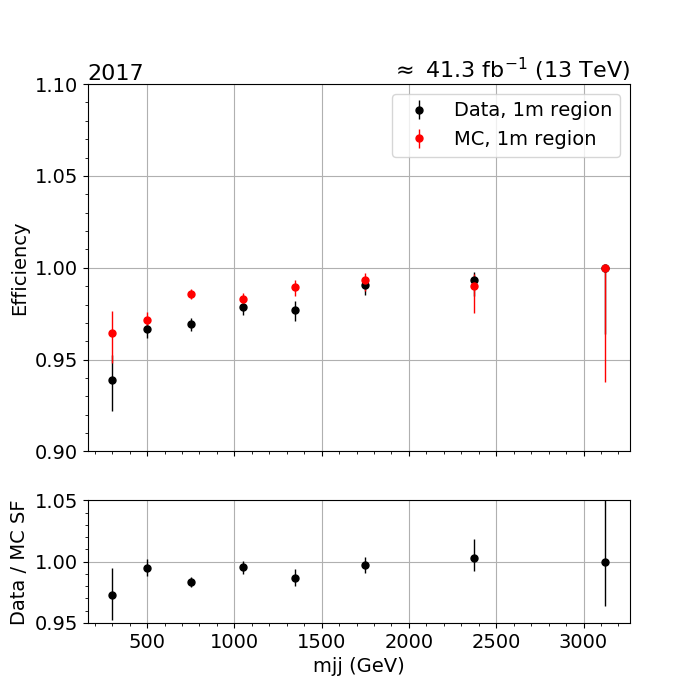
\includegraphics[width=0.49\textwidth]{fig/efficiency/trigger/met/mjj/data_mc_comparison_1m_2017_one_jet_forward_one_jet_central.png}
        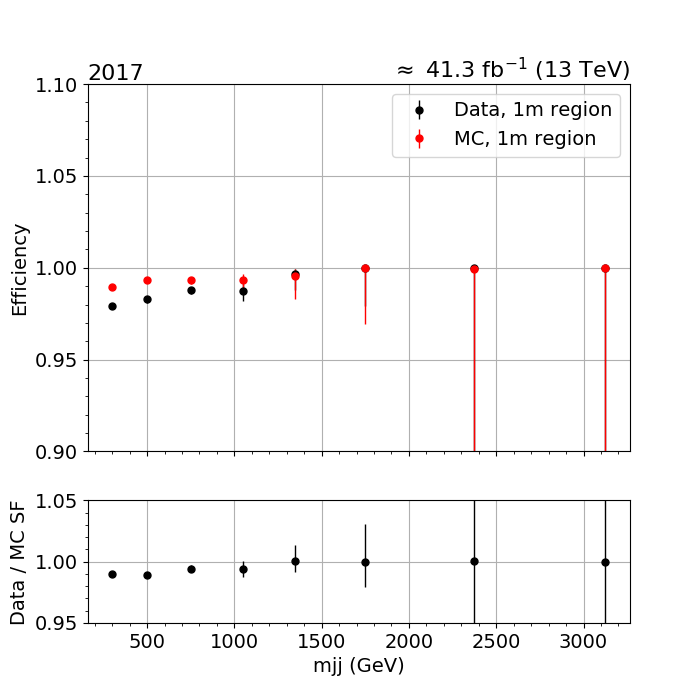
\includegraphics[width=0.49\textwidth]{fig/efficiency/trigger/met/mjj/data_mc_comparison_1m_2017_two_central_jets.png} \\
        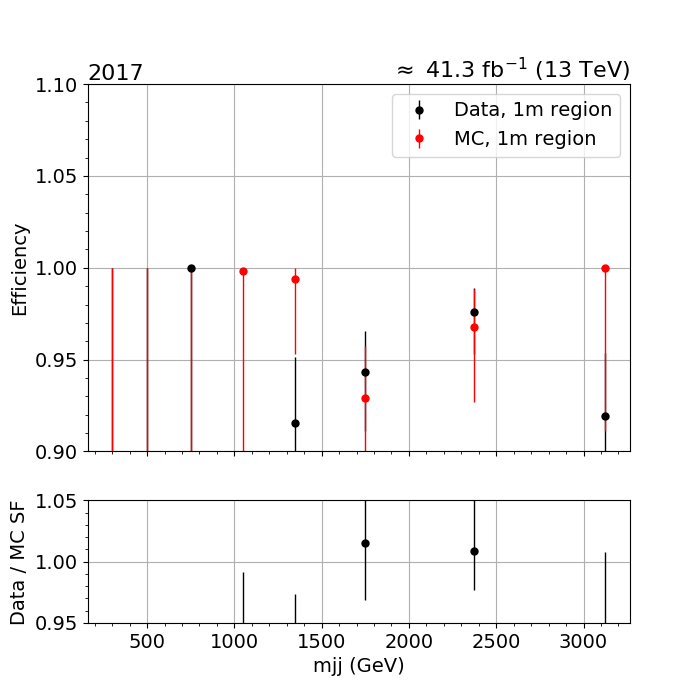
\includegraphics[width=0.49\textwidth]{fig/efficiency/trigger/met/mjj/data_mc_comparison_1m_2017_two_forward_jets.png}
    \end{center}
    \caption{MET trigger efficiency as a function of mjj in three categories: One forward jet and one central jet, two central jets and
            two forward jets. These results are obtained from 2017 data and MC samples with the selection of single muon events.} 
    \label{fig:eff_mjj_2017_1m}      
\end{figure}

\begin{figure}[hbp]
    \begin{center}
        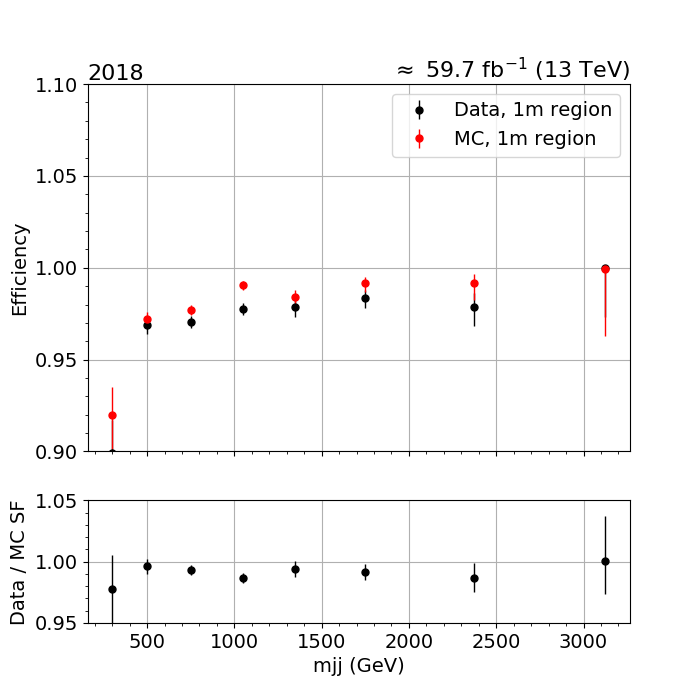
\includegraphics[width=0.49\textwidth]{fig/efficiency/trigger/met/mjj/data_mc_comparison_1m_2018_one_jet_forward_one_jet_central.png}
        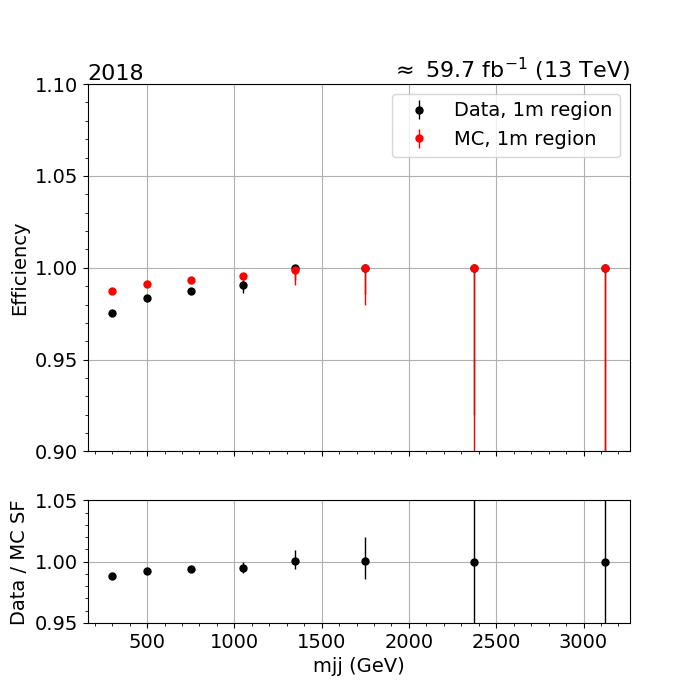
\includegraphics[width=0.49\textwidth]{fig/efficiency/trigger/met/mjj/data_mc_comparison_1m_2018_two_central_jets.png} \\
        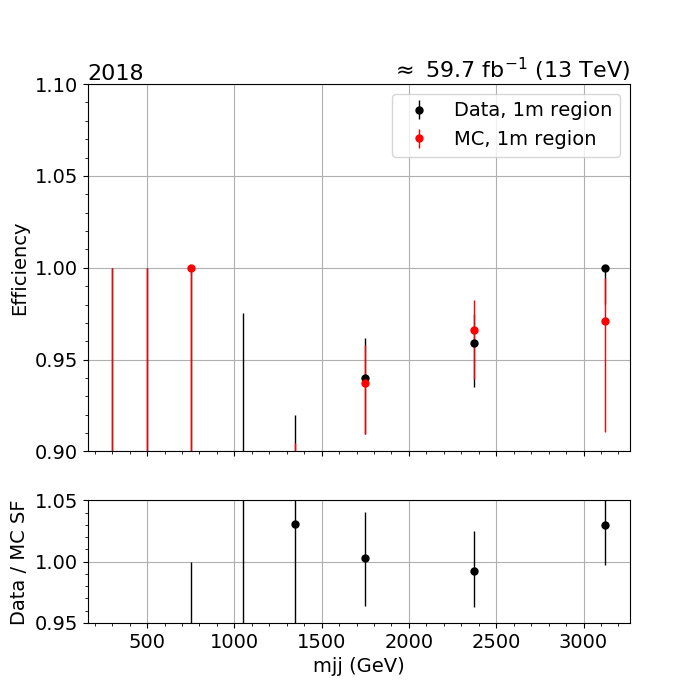
\includegraphics[width=0.49\textwidth]{fig/efficiency/trigger/met/mjj/data_mc_comparison_1m_2018_two_forward_jets.png}
    \end{center}
    \caption{MET trigger efficiency as a function of mjj in three categories: One forward jet and one central jet, two central jets and
            two forward jets. These results are obtained from 2018 data and MC samples with the selection of single muon events.}   
    \label{fig:eff_mjj_2018_1m}
\end{figure}

Figs.~\ref{fig:eff_recoil_2017_2m} and ~\ref{eff_recoil_2018_2m} show the efficiencies obtained in double muon CR 
as a function of recoil in data and MC for the three jet categories in 2017 and 2018, respectively. 
Figs.~\ref{fig:eff_mjj_2017_2m} and ~\ref{eff_mjj_2018_2m} show the efficiencies obtained in double muon CR 
as a function of $\mjj$ in data and MC for the three jet categories in 2017 and 2018, respectively. 

\begin{figure}[htp]
    \begin{center}
        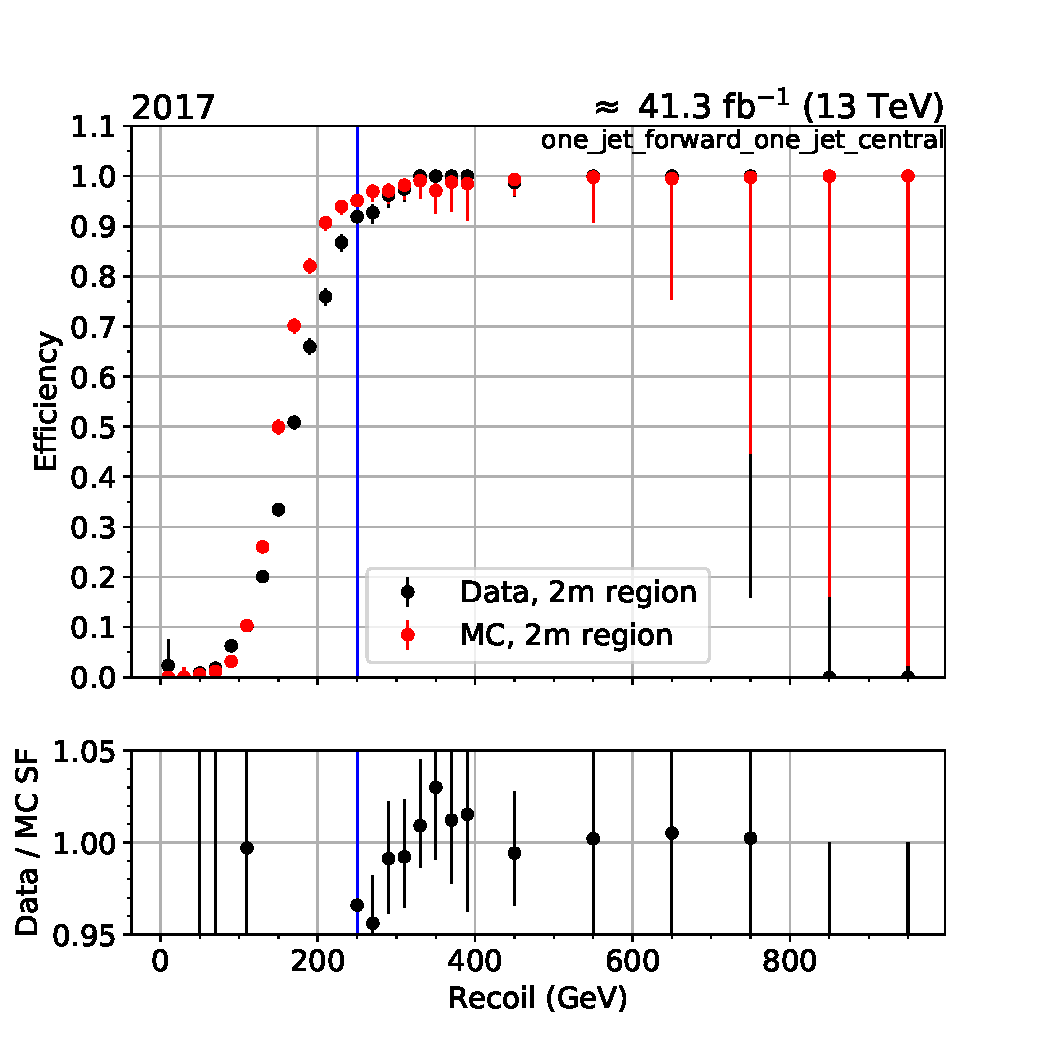
\includegraphics[width=0.49\textwidth]{fig/efficiency/trigger/met/recoil/data_mc_comparison_2m_2017_one_jet_forward_one_jet_central.pdf}
        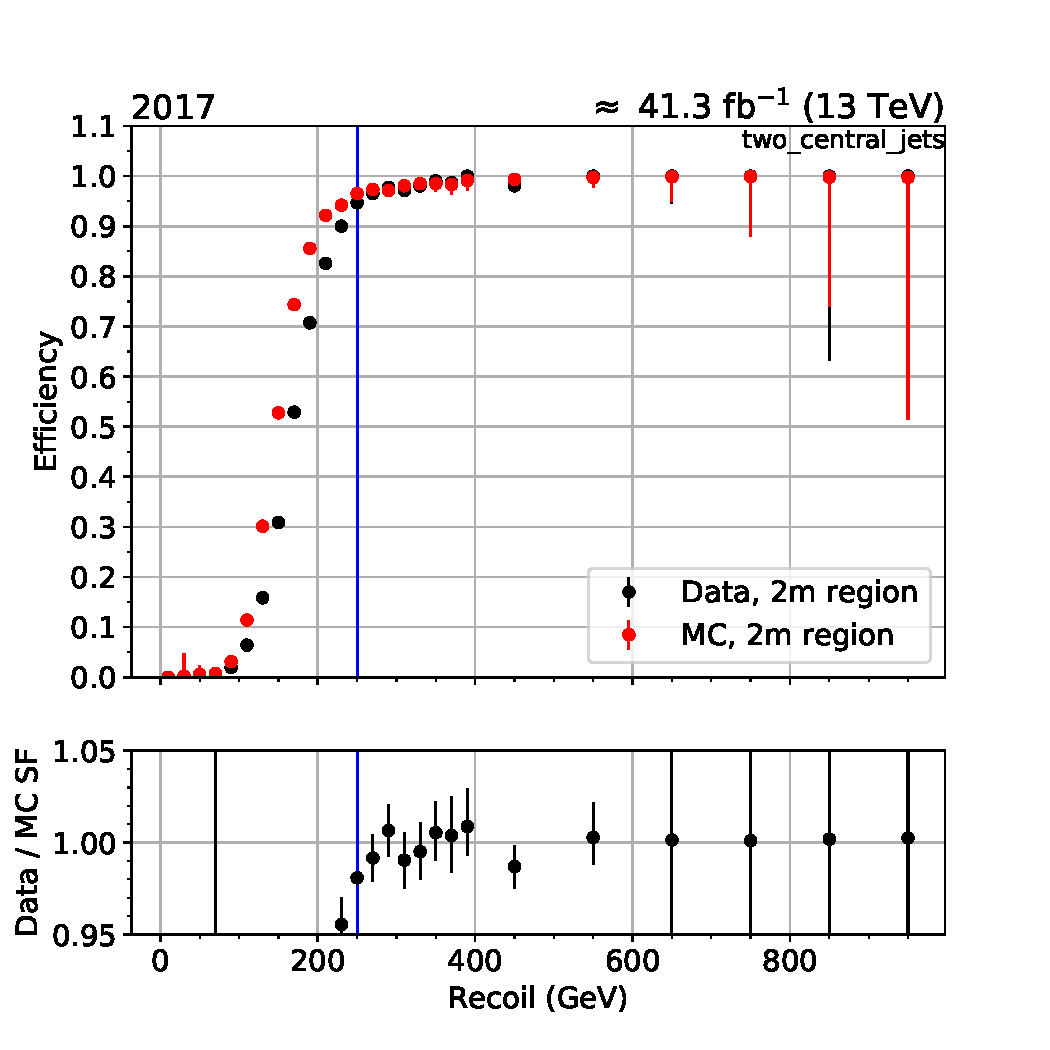
\includegraphics[width=0.49\textwidth]{fig/efficiency/trigger/met/recoil/data_mc_comparison_2m_2017_two_central_jets.pdf} \\
        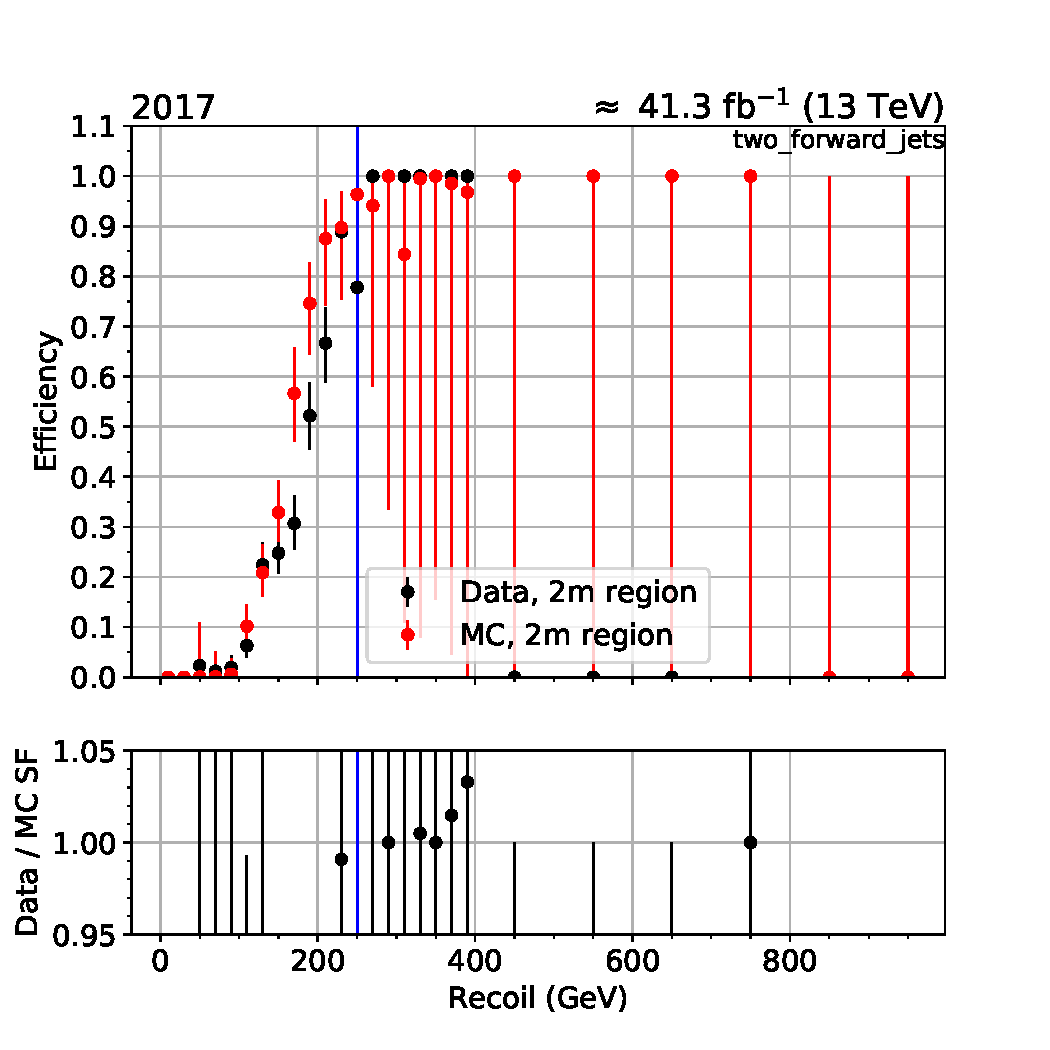
\includegraphics[width=0.49\textwidth]{fig/efficiency/trigger/met/recoil/data_mc_comparison_2m_2017_two_forward_jets.pdf}
    \end{center}
    \caption{MET trigger efficiency as a function of recoil in three categories: One forward jet and one central jet, two central jets and
            two forward jets. These results are obtained from 2017 data and MC samples with the selection of double muon events.} 
    \label{fig:eff_recoil_2017_2m}      
\end{figure}

\begin{figure}[htp]
    \begin{center}
        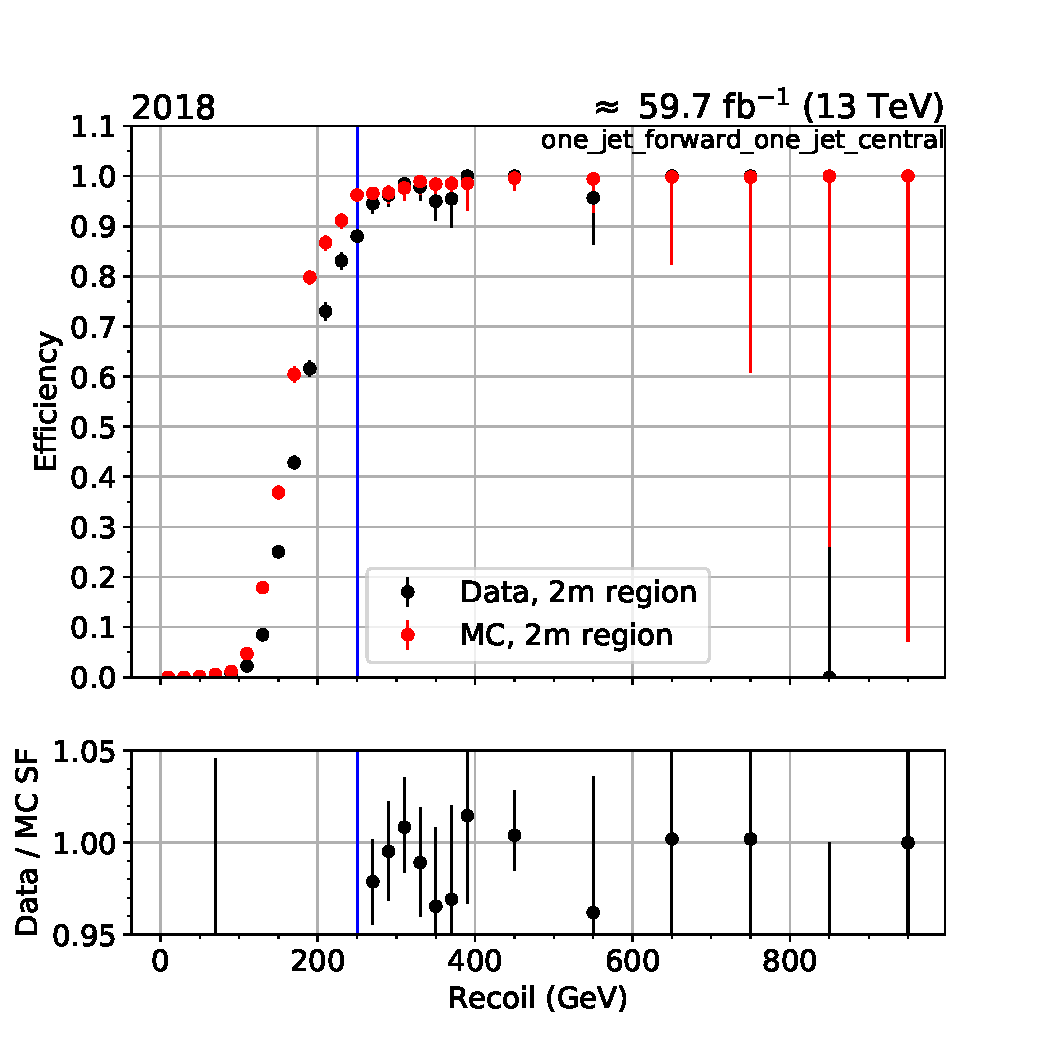
\includegraphics[width=0.49\textwidth]{fig/efficiency/trigger/met/recoil/data_mc_comparison_2m_2018_one_jet_forward_one_jet_central.pdf}
        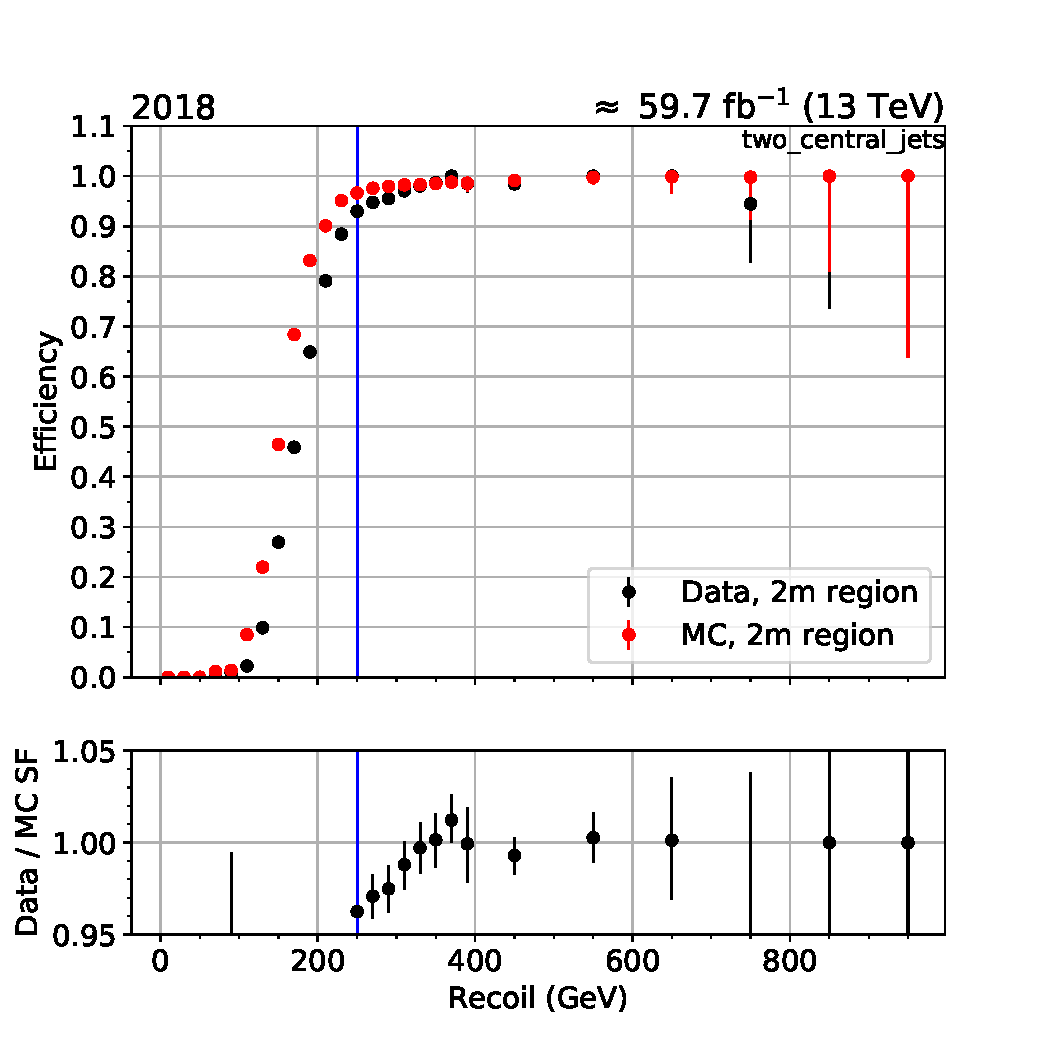
\includegraphics[width=0.49\textwidth]{fig/efficiency/trigger/met/recoil/data_mc_comparison_2m_2018_two_central_jets.pdf} \\
        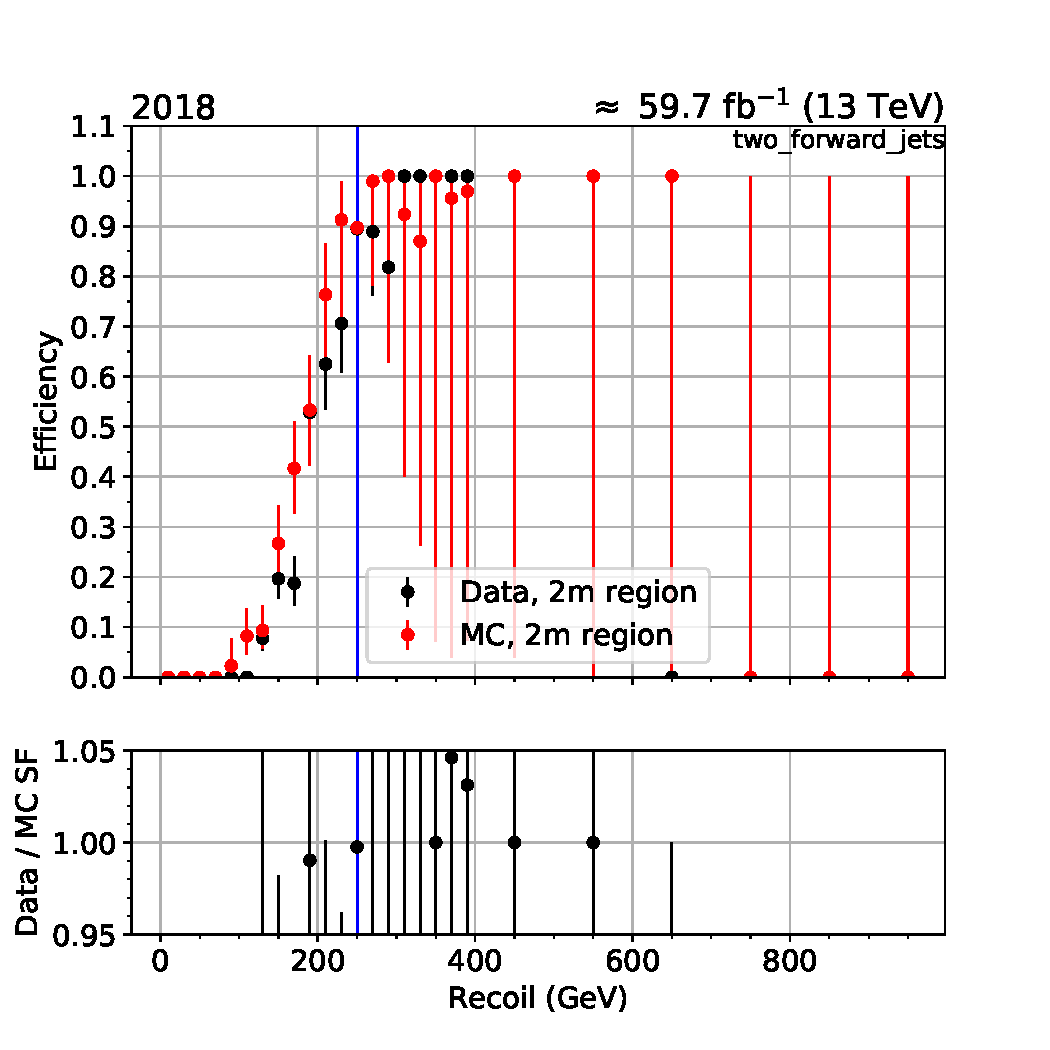
\includegraphics[width=0.49\textwidth]{fig/efficiency/trigger/met/recoil/data_mc_comparison_2m_2018_two_forward_jets.pdf}
    \end{center}
    \caption{MET trigger efficiency as a function of recoil in three categories: One forward jet and one central jet, two central jets and
            two forward jets. These results are obtained from 2018 data and MC samples with the selection of double muon events.} 
    \label{fig:eff_recoil_2018_2m}      
\end{figure}

\begin{figure}[htp]
    \begin{center}
        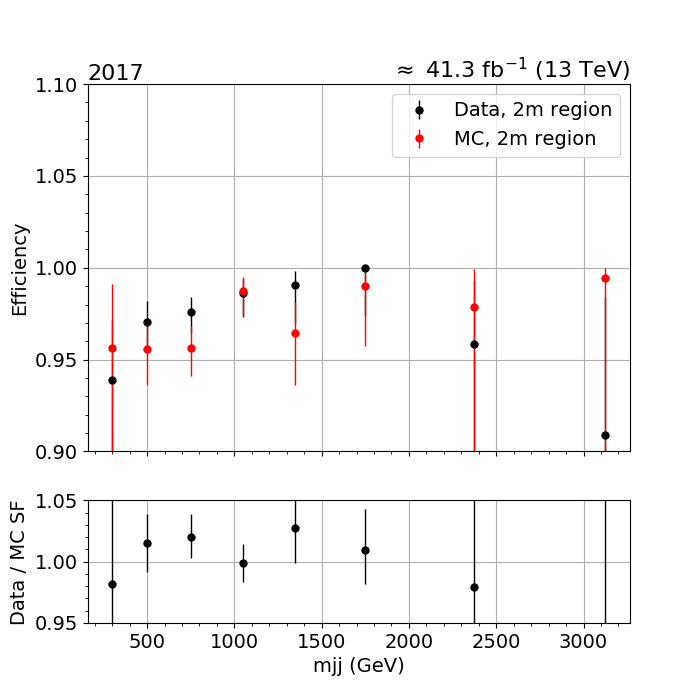
\includegraphics[width=0.49\textwidth]{fig/efficiency/trigger/met/mjj/data_mc_comparison_2m_2017_one_jet_forward_one_jet_central.png}
        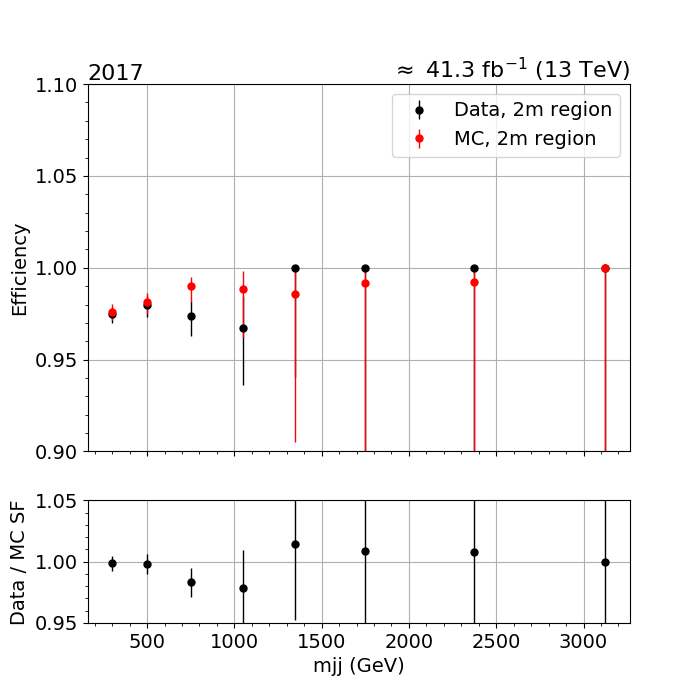
\includegraphics[width=0.49\textwidth]{fig/efficiency/trigger/met/mjj/data_mc_comparison_2m_2017_two_central_jets.png} \\
        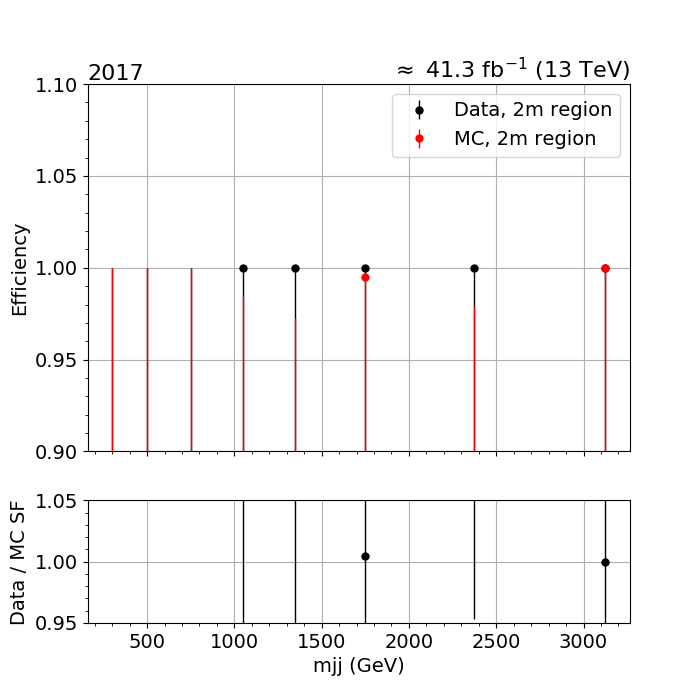
\includegraphics[width=0.49\textwidth]{fig/efficiency/trigger/met/mjj/data_mc_comparison_2m_2017_two_forward_jets.png}
    \end{center}
    \caption{MET trigger efficiency as a function of mjj in three categories: One forward jet and one central jet, two central jets and
            two forward jets. These results are obtained from 2017 data and MC samples with the selection of double muon events.} 
    \label{fig:eff_mjj_2017_2m}      
\end{figure}

\begin{figure}[htp]
    \begin{center}
        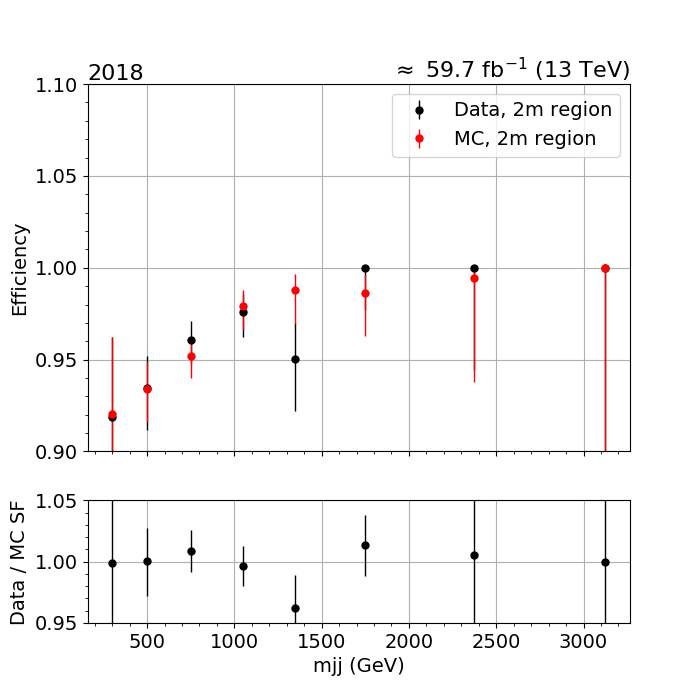
\includegraphics[width=0.49\textwidth]{fig/efficiency/trigger/met/mjj/data_mc_comparison_2m_2018_one_jet_forward_one_jet_central.png}
        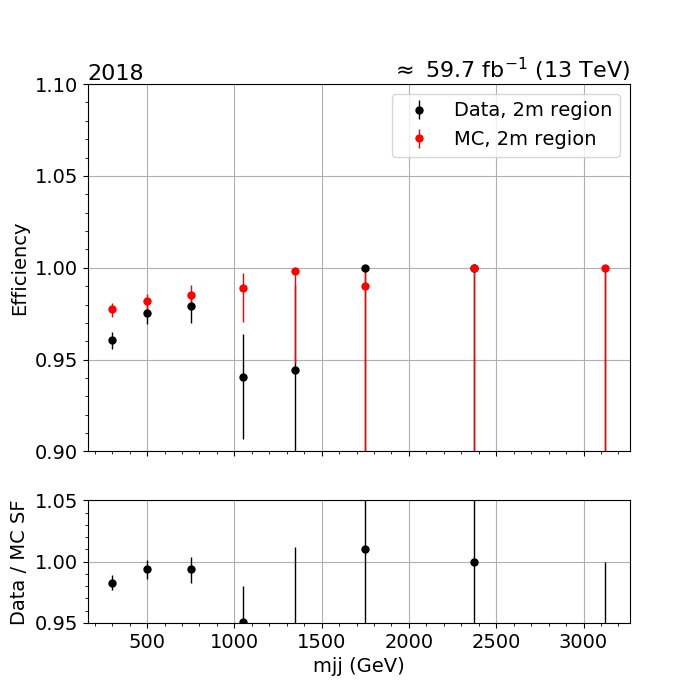
\includegraphics[width=0.49\textwidth]{fig/efficiency/trigger/met/mjj/data_mc_comparison_2m_2018_two_central_jets.png} \\
        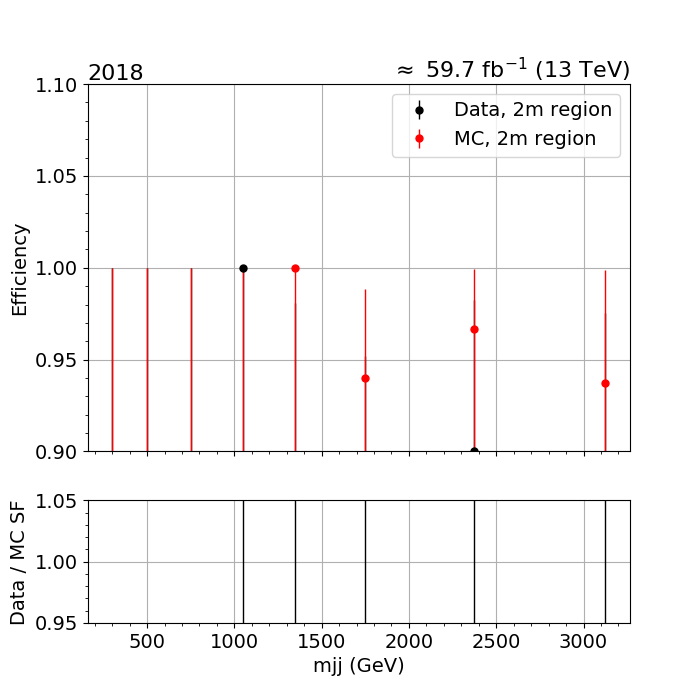
\includegraphics[width=0.49\textwidth]{fig/efficiency/trigger/met/mjj/data_mc_comparison_2m_2018_two_forward_jets.png}
    \end{center}
    \caption{MET trigger efficiency as a function of mjj in three categories: One forward jet and one central jet, two central jets and
            two forward jets. These results are obtained from 2018 data and MC samples with the selection of double muon events.} 
    \label{fig:eff_mjj_2018_2m}      
\end{figure}

Fig.~\ref{fig:sf_recoil_2m} shows the scale factors as a function of recoil in double muon control region, using 2017 (left)
and 2018 (right) samples. 

\begin{figure}[hbp]
    \begin{center}
        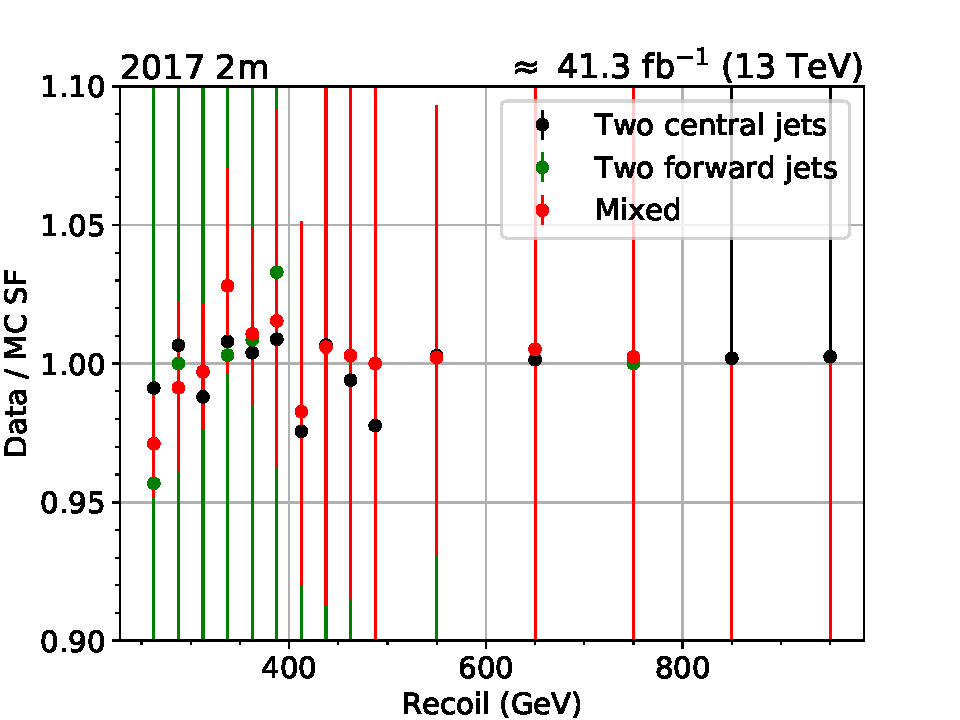
\includegraphics[width=0.49\textwidth]{fig/efficiency/trigger/met/recoil/scale_factors_2m_2017.pdf}
        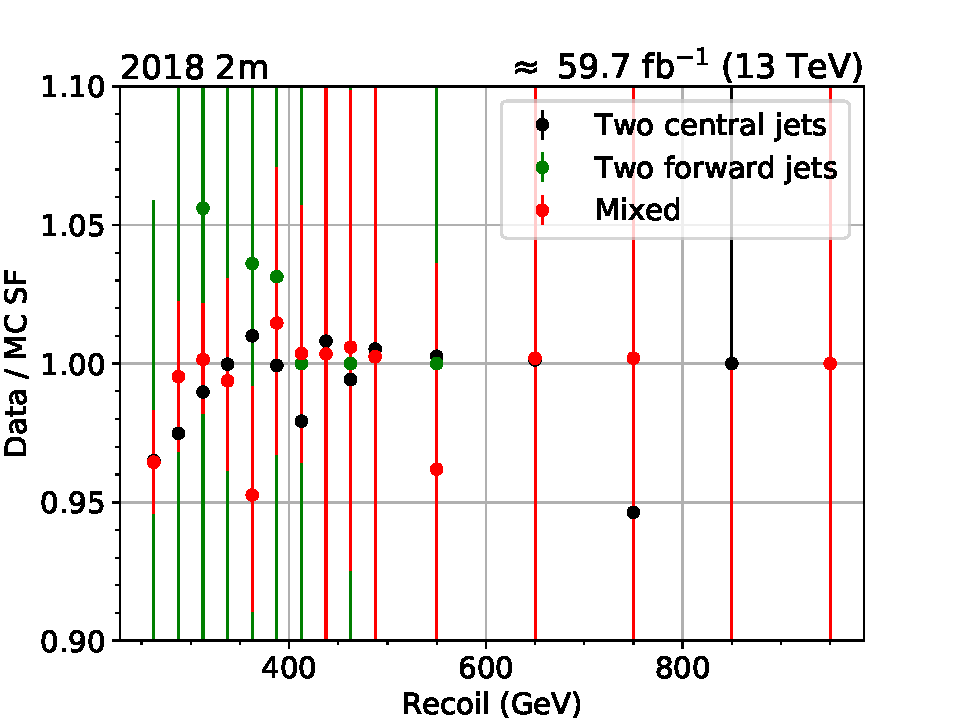
\includegraphics[width=0.49\textwidth]{fig/efficiency/trigger/met/recoil/scale_factors_2m_2018.pdf} 
    \end{center}
    \caption{Data-MC scale factors for the three jet kinematic cases in the double muon control region, using 2017 (left) and 2018 (right) samples.}
    \label{fig:sf_recoil_2m}
\end{figure}

